\documentclass[aspectratio=169,11pt]{beamer}

\usepackage{iftex}
\ifXeTeX
  \usepackage{fontspec}
  % For Chinese, replace the fallback with an installed CJK font.
  % The builder rejects missing-glyph warnings.
  \IfFontExistsTF{Noto Sans CJK SC}
    {\setmainfont{Noto Sans CJK SC}\setsansfont{Noto Sans CJK SC}}
    {\setmainfont{Latin Modern Sans}\setsansfont{Latin Modern Sans}}
\else
  \PackageError{slides}{Compile with XeLaTeX}{Use the supplied builder}
\fi

\usepackage{amsmath,amssymb,booktabs,graphicx,tikz}
\usepackage[round,authoryear]{natbib}
\graphicspath{{figures/}}

\usetheme{default}
\setbeamertemplate{navigation symbols}{}
\setbeamertemplate{footline}[frame number]
\setbeamertemplate{frametitle continuation}{}
\setbeamertemplate{itemize items}[circle]
\setbeamertemplate{blocks}[rounded][shadow=false]

\definecolor{Ink}{HTML}{172033}
\definecolor{Accent}{HTML}{176B87}
\definecolor{Warm}{HTML}{D97B29}
\definecolor{Mist}{HTML}{F3F6F8}
\setbeamercolor{normal text}{fg=Ink,bg=white}
\setbeamercolor{structure}{fg=Accent}
\setbeamercolor{frametitle}{fg=Ink,bg=white}
\setbeamercolor{block title}{fg=white,bg=Accent}
\setbeamercolor{block body}{fg=Ink,bg=Mist}

\title{Paper title}
\subtitle{Reading-group presentation}
\author{Presenter}
\institute{Institution}
\date{\today}

% Optional: commands used only inside \note or \speech.
\NotesPreamble{
  % \newcommand{\solver}{branch-and-cut solver}
}

\begin{document}

\begin{paperframe}[plain]{S01}{}
  \titlepage
\end{paperframe}
\note{Check the title, authors, venue, and pronunciation before starting.}
\speech{Introduce the paper, the reading-group context, and the central question. Suggested time: 30 seconds.}

\begin{paperframe}{S02}{What kind of paper is this?}
  \begin{block}{Paper identity}
    Survey, original method, empirical study, tutorial, benchmark, or position paper
  \end{block}
  \begin{itemize}
    \item Central question
    \item Authors' actual contribution
    \item Scope and evidence boundary
  \end{itemize}
\end{paperframe}
\note{Do not attribute prior algorithms to survey authors.}
\speech{Classify the paper from its evidence, then distinguish the authors' contribution from the work they summarize. Suggested time: 60 seconds.}

\begin{paperframe}{S03}{Prerequisites: Core concepts}
  \begin{columns}[T]
    \begin{column}{0.48\textwidth}
      \begin{block}{Concept A}Plain-language definition\end{block}
    \end{column}
    \begin{column}{0.48\textwidth}
      \begin{block}{Concept B}Relationship to Concept A\end{block}
    \end{column}
  \end{columns}
\end{paperframe}
\note{Use a concrete object and action for each concept.}
\speech{Explain the prerequisite hierarchy and give one small example that can be spoken without reading the slide. Suggested time: 90 seconds.}

\begin{paperframe}{S04}{Method: Input, decision, and output}
  \centering
  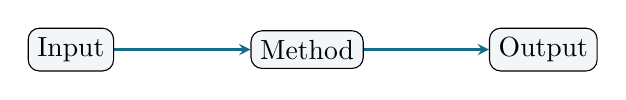
\begin{tikzpicture}[node distance=1.8cm,>=stealth]
    \node[draw,rounded corners,fill=Mist] (input) {Input};
    \node[draw,rounded corners,fill=Mist,right of=input,xshift=1.2cm] (method) {Method};
    \node[draw,rounded corners,fill=Mist,right of=method,xshift=1.2cm] (output) {Output};
    \draw[->,thick,Accent] (input) -- (method);
    \draw[->,thick,Accent] (method) -- (output);
  \end{tikzpicture}
  \vfill
  {\small Add a citation near the claim: \citep{paper}}
\end{paperframe}
\note{Name the exact input objects, decision, and downstream use.}
\speech{Walk from input through transformation to output. Add a practical benefit, limitation, and transition. Suggested time: 120 seconds.}

\begin{paperframe}{S05}{Takeaways}
  \begin{enumerate}
    \item What the paper contributes
    \item What the evidence supports
    \item What remains limited or open
  \end{enumerate}
\end{paperframe}
\note{End on the evidence boundary, not a stronger claim.}
\speech{Restate the contribution, evidence, and open question in one sentence each. Suggested time: 60 seconds.}

\begin{paperframe}{S06}{References}
  \bibliographystyle{apalike}
  \bibliography{references}
\end{paperframe}
\note{Keep this page available for questions.}
\speech{Thank the audience and invite questions. Suggested time: 15 seconds.}

\end{document}
